\section{Nền tảng Kiến trúc}
\label{sec:cnn_architecture_fundamentals}

Kiến trúc Mạng Nơ-ron Tích chập, dù có vẻ phức tạp với nhiều biến thể hiện đại, thực chất được xây dựng từ một vài khối chức năng (functional blocks) cơ bản, được xếp chồng lên nhau để tạo thành một hệ thống xử lý thông tin phân cấp. Việc hiểu rõ từng khối xây dựng này—chức năng riêng của chúng, các tham số điều khiển, và lý do toán học đằng sau sự tồn tại của chúng—là điều kiện tiên quyết để có thể làm chủ CNN.

Trong phần này, chúng ta sẽ mổ xẻ ba thành phần cốt lõi tạo nên hầu hết các lớp trong một mạng CNN:
\begin{enumerate}
	\item \textbf{Lớp Tích chập (Convolutional Layer):} Trái tim của mạng, nơi thực hiện việc trích xuất đặc trưng.
	\item \textbf{Lớp Gộp (Pooling Layer):} Cơ chế giảm chiều không gian và tạo ra tính bất biến.
	\item \textbf{Hàm Kích hoạt (Activation Function):} Thành phần đưa tính phi tuyến vào mạng, cho phép học các mối quan hệ phức tạp.
\end{enumerate}

Chúng ta sẽ bắt đầu với phép toán đã đặt tên cho toàn bộ kiến trúc: phép tích chập.

\subsection{Convolution: Cơ chế Trượt và Nhân Tích chập}
\label{subsec:convolution_mechanism}

Ở Chương 2, chúng ta đã làm quen với các bộ lọc thủ công như Sobel hay Laplacian để phát hiện cạnh. Các bộ lọc này về bản chất là những ma trận số nhỏ (gọi là \textbf{kernel} hoặc \textbf{bộ lọc}), được trượt qua toàn bộ ảnh. Tại mỗi vị trí, chúng ta thực hiện một phép nhân theo từng phần tử (element-wise multiplication) giữa kernel và vùng ảnh bên dưới nó, sau đó tính tổng để ra một giá trị pixel duy nhất ở ảnh đầu ra.

Phép toán này chính là \textbf{tích chập 2D (2D Convolution)}.

Điểm khác biệt mang tính cách mạng của CNN là: \textbf{Thay vì sử dụng các kernel với các giá trị được thiết kế thủ công, CNN coi các giá trị trong kernel là các tham số có thể học được (learnable parameters)}. Mạng sẽ tự động học các giá trị của kernel để phát hiện ra những đặc trưng hữu ích nhất cho tác vụ đang cần giải quyết, thông qua quá trình huấn luyện với thuật toán lan truyền ngược.

\subsubsection{Cơ chế Hoạt động: "Cửa sổ trượt" Feature Detector}
\label{subsubsec:conv_sliding_window}
Hãy hình dung một kernel như một "cửa sổ" hay một "đèn pin" nhỏ trượt trên bề mặt của ảnh đầu vào. Cửa sổ này có nhiệm vụ tìm kiếm một loại "pattern" (mẫu) cụ thể.
\begin{itemize}
	\item \textbf{Ảnh đầu vào (Input Image/Feature Map):} Một ma trận số, có thể là ảnh gốc (ví dụ: $32 \times 32 \times 3$) hoặc một bản đồ đặc trưng (feature map) từ lớp trước đó.
	\item \textbf{Kernel (hoặc Bộ lọc - Filter):} Một ma trận số nhỏ hơn nhiều so với ảnh đầu vào (ví dụ: $5 \times 5 \times 3$). Đây chính là bộ phát hiện đặc trưng (feature detector). Các giá trị trong kernel định nghĩa loại pattern mà nó đang tìm kiếm.
	\item \textbf{Bản đồ Đặc trưng Đầu ra (Output Feature Map / Activation Map):} Kết quả của phép tích chập. Mỗi pixel trên bản đồ này cho biết mức độ "kích hoạt" (response) của kernel tại vị trí tương ứng trên ảnh đầu vào. Một giá trị cao có nghĩa là pattern mà kernel tìm kiếm đã được tìm thấy.
\end{itemize}

Quá trình tính toán cho một vị trí trên bản đồ đầu ra diễn ra như sau:
\begin{enumerate}
	\item Đặt kernel lên góc trên cùng bên trái của ảnh đầu vào.
	\item Thực hiện phép nhân theo từng phần tử giữa các giá trị của kernel và các giá trị pixel của ảnh nằm bên dưới nó.
	\item Tính tổng tất cả các kết quả của phép nhân ở bước 2. Kết quả tổng này là giá trị của pixel đầu tiên (góc trên trái) của bản đồ đặc trưng đầu ra.
	\item Dịch chuyển kernel sang phải một khoảng nhất định (gọi là \textit{stride}), và lặp lại các bước 2-3.
	\item Lặp lại quá trình cho đến khi kernel trượt hết toàn bộ ảnh đầu vào.
\end{enumerate}

\begin{center}
	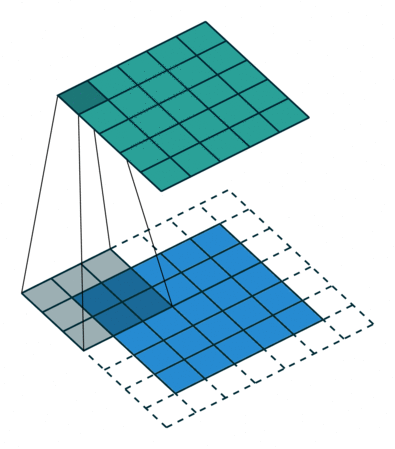
\includegraphics[width=1.0\textwidth]{images/convolution_sliding_window_animation.png}
	\captionof{figure}{Minh họa cơ chế tích chập 2D. Kernel màu xanh lá cây ($3 \times 3$) trượt trên ảnh đầu vào màu xanh dương ($5 \times 5$). Tại mỗi vị trí, một phép nhân tích chập được thực hiện để tạo ra một giá trị trong bản đồ đặc trưng đầu ra.}
	\label{fig:convolution_sliding_window}
\end{center}

\subsubsection{Công thức Toán học}
\label{subsubsec:conv_math_formula}
Đối với một ảnh đầu vào $I$ và một kernel $K$, giá trị tại vị trí $(i, j)$ của bản đồ đặc trưng đầu ra $O$ được tính bởi công thức tích chập 2D rời rạc:
\begin{equation}
	O(i, j) = (I * K)(i, j) = \sum_{m} \sum_{n} I(i-m, j-n) K(m, n)
	\label{eq:convolution_formula}
\end{equation}
Trong thực tế tính toán của các thư viện học sâu, phép toán thường được triển khai dưới dạng \textbf{tương quan chéo (cross-correlation)}, trong đó kernel không bị lật:
\begin{equation}
	O(i, j) = (I \star K)(i, j) = \sum_{m} \sum_{n} I(i+m, j+n) K(m, n)
	\label{eq:cross_correlation_formula}
\end{equation}
Vì các giá trị trong kernel $K$ đều được học, việc lật kernel hay không không tạo ra sự khác biệt về khả năng biểu diễn của mạng. Do đó, trong bối cảnh CNN, thuật ngữ "tích chập" gần như luôn luôn ám chỉ phép tương quan chéo vì nó đơn giản hơn để triển khai.

\subsubsection{Trực quan hóa vai trò của Kernel}
\label{subsubsec:conv_kernel_visualization}
Một kernel $3 \times 3$ có thể được thiết kế để phát hiện các cạnh đơn giản. Ví dụ:
\[
K_{\text{vertical}} = 
\begin{pmatrix}
	1 & 0 & -1 \\
	1 & 0 & -1 \\
	1 & 0 & -1
\end{pmatrix}
\quad
K_{\text{horizontal}} = 
\begin{pmatrix}
	1 & 1 & 1 \\
	0 & 0 & 0 \\
	-1 & -1 & -1
\end{pmatrix}
\]
Khi trượt kernel $K_{\text{vertical}}$ qua ảnh, nó sẽ cho giá trị dương lớn ở những nơi có sự chuyển tiếp từ sáng sang tối theo chiều ngang (cạnh dọc), giá trị âm lớn ở những nơi có sự chuyển tiếp từ tối sang sáng, và giá trị gần bằng 0 ở các vùng phẳng hoặc trên các cạnh ngang.

Trong CNN, mạng không được cho trước các kernel này. Thay vào đó, nó tự học các giá trị tối ưu cho hàng chục, hàng trăm kernel khác nhau. Các lớp đầu tiên thường học các kernel phát hiện các đặc trưng nguyên thủy như cạnh, góc, và các đốm màu.

\begin{center}
	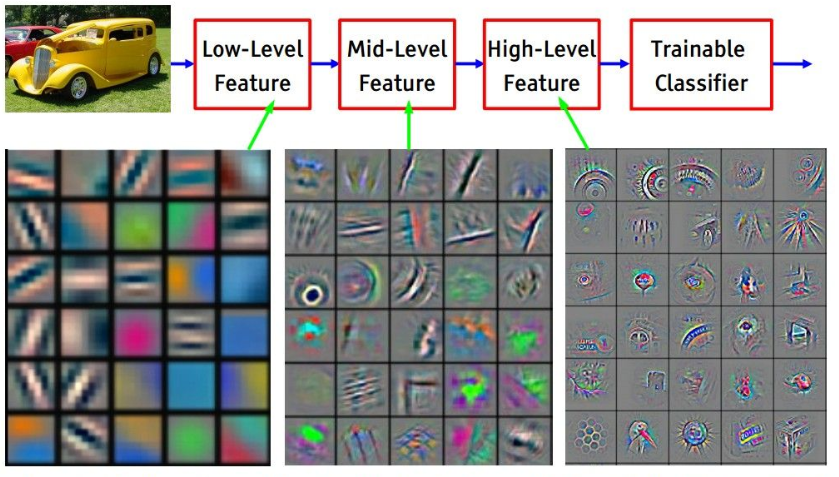
\includegraphics[width=0.8\textwidth]{images/cnn_filter_visualization.png}
	\captionof{figure}{Vai trò của kernel như một bộ phát hiện pattern. Mỗi kernel được học để kích hoạt (cho ra giá trị cao) khi nó "nhìn thấy" một loại pattern cụ thể trong vùng ảnh đầu vào.}
	\label{fig:cnn_filter_visualization}
\end{center}
% Keyword gợi ý: cnn filter visualization, what cnn kernels learn, cnn feature detector

\subsubsection{Từ Grayscale đến RGB và các Chiều sâu}
\label{subsubsec:conv_depth_channels}
Một hình ảnh thực tế thường có nhiều kênh màu (ví dụ: 3 kênh R, G, B). Khái niệm tích chập được mở rộng một cách tự nhiên để xử lý các input đa kênh này.

\begin{description}
	\item[Input đa kênh:] Nếu ảnh đầu vào có kích thước $W_{in} \times H_{in} \times C_{in}$ (ví dụ: $32 \times 32 \times 3$), thì kernel cũng phải có cùng chiều sâu, tức là kích thước của nó sẽ là $F \times F \times C_{in}$ (ví dụ: $5 \times 5 \times 3$).
	\item[Phép toán 3D:] Phép nhân tích chập lúc này diễn ra trên toàn bộ khối 3D. Kernel $5 \times 5 \times 3$ được đặt lên một vùng $5 \times 5 \times 3$ của ảnh đầu vào, thực hiện $5 \times 5 \times 3 = 75$ phép nhân, sau đó tất cả được cộng lại để tạo ra \textbf{một giá trị duy nhất} trên bản đồ đầu ra.
	\item[Output 2D:] Điều quan trọng cần lưu ý là, dù kernel và input có chiều sâu, kết quả của một phép tích chập với \textbf{một kernel} luôn là một bản đồ đặc trưng \textbf{2D} (một kênh).
\end{description}

\begin{mdframed}[style=infobox]
	\textbf{Trực giác: Kernel 3D học các pattern màu sắc}
	
	Một kernel $5 \times 5 \times 3$ không còn chỉ là một bộ phát hiện hình dạng, mà nó còn là một bộ phát hiện \textbf{hình dạng + màu sắc}. Ví dụ, một kernel có thể học cách phát hiện một cạnh dọc có màu đỏ ở bên trái và màu xanh lá ở bên phải. Nó thực hiện điều này bằng cách có các giá trị dương lớn ở các vị trí tương ứng trong kênh màu đỏ, và các giá trị âm lớn ở các vị trí tương ứng trong kênh màu xanh lá.
\end{mdframed}

\subsubsection{Sử dụng nhiều Kernel để tạo ra Output đa kênh}
\label{subsubsec:conv_multiple_filters}
Nếu một kernel chỉ có thể phát hiện một loại đặc trưng, làm thế nào để mạng có thể phát hiện nhiều loại đặc trưng khác nhau cùng lúc (ví dụ: cạnh dọc, cạnh ngang, cạnh xiên, màu xanh, màu đỏ,...)?

Câu trả lời là sử dụng nhiều kernel trong cùng một lớp tích chập.
\begin{itemize}
	\item Mỗi kernel trong lớp sẽ được khởi tạo ngẫu nhiên và trong quá trình huấn luyện, nó sẽ tự chuyên biệt hóa để phát hiện một loại pattern khác nhau.
	\item Mỗi kernel sẽ tạo ra một bản đồ đặc trưng 2D riêng biệt.
	\item Các bản đồ đặc trưng này sau đó được xếp chồng lên nhau để tạo thành một khối output (output volume).
\end{itemize}
Nếu một lớp tích chập có $C_{out}$ kernel (bộ lọc), thì output của lớp đó sẽ có chiều sâu là $C_{out}$.

Tóm lại, một lớp tích chập hoàn chỉnh thực hiện phép biến đổi từ một khối input $W_{in} \times H_{in} \times C_{in}$ thành một khối output $W_{out} \times H_{out} \times C_{out}$ bằng cách sử dụng $C_{out}$ bộ lọc, mỗi bộ lọc có kích thước $F \times F \times C_{in}$.

\begin{center}
	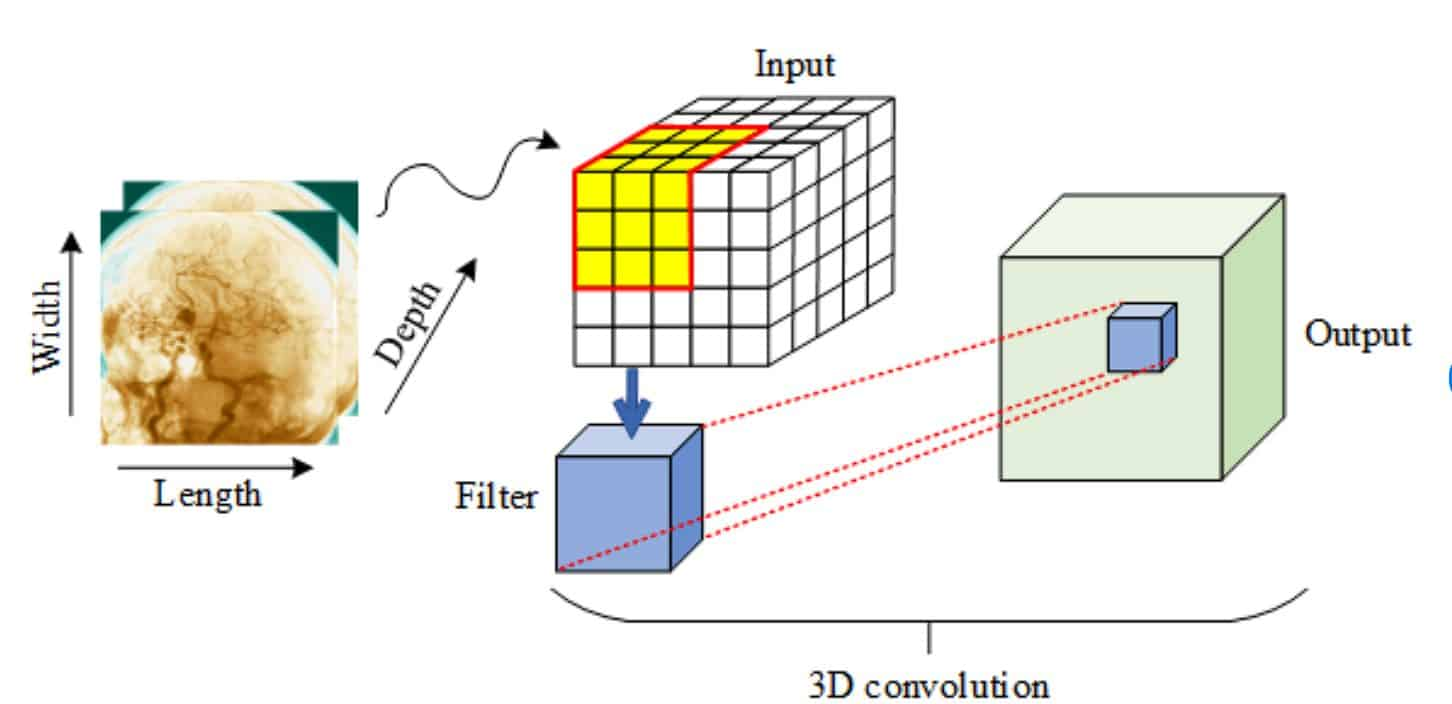
\includegraphics[width=1.0\textwidth]{images/convolution_layer_3d_volume.jpg}
	\captionof{figure}{Hoạt động của một lớp tích chập đầy đủ. Input có chiều sâu $C_{in}$. Lớp tích chập sử dụng $C_{out}$ bộ lọc (mỗi bộ lọc cũng có chiều sâu $C_{in}$) để tạo ra một khối output có chiều sâu $C_{out}$.}
	\label{fig:convolution_3d_volume}
\end{center}

\subsubsection{Các Siêu tham số của Lớp Tích chập}
\label{subsubsec:conv_hyperparameters}
Bên cạnh các giá trị của kernel (là các tham số học được), một lớp tích chập được định nghĩa bởi một vài siêu tham số (hyperparameters) do người thiết kế mạng quyết định. Chúng kiểm soát hành vi và kích thước đầu ra của lớp.

\begin{description}
	\item[Kích thước Kernel (Kernel Size - F):] Kích thước của bộ lọc (ví dụ: $3 \times 3$, $5 \times 5$, $7 \times 7$). Kernel nhỏ hơn ($3 \times 3$) có trường thụ cảm (receptive field) nhỏ, tập trung vào các đặc trưng rất cục bộ. Kernel lớn hơn có thể nắm bắt các pattern phức tạp hơn. Trong các kiến trúc hiện đại, người ta ưa chuộng sử dụng nhiều lớp tích chập với kernel $3 \times 3$ xếp chồng lên nhau thay vì một lớp với kernel lớn, vì nó hiệu quả hơn về tham số và có tính phi tuyến cao hơn.
	
	\item[Sải bước (Stride - S):] Khoảng cách mà kernel dịch chuyển trên ảnh đầu vào sau mỗi lần tính toán. Stride bằng 1 (mặc định) có nghĩa là kernel trượt đi từng pixel một, tạo ra một bản đồ đầu ra có kích thước gần bằng đầu vào. Stride lớn hơn 1 (ví dụ: $S=2$) sẽ làm cho kernel "nhảy" các pixel, dẫn đến một bản đồ đầu ra nhỏ hơn đáng kể (downsampling). Đây là một cách để giảm kích thước không gian của dữ liệu.
	
	\item[Đệm (Padding - P):] Khi áp dụng kernel ở các rìa của ảnh, một phần của kernel sẽ nằm ngoài ảnh. Để xử lý việc này và để kiểm soát kích thước của bản đồ đầu ra, người ta thường "đệm" (pad) các đường viền của ảnh đầu vào bằng các giá trị 0. Một kỹ thuật phổ biến là \textbf{"same" padding}, trong đó giá trị P được chọn sao cho kích thước chiều rộng và chiều cao của bản đồ đầu ra bằng với bản đồ đầu vào (khi $S=1$). Nếu không có padding ($P=0$), bản đồ đầu ra sẽ bị co lại một chút sau mỗi lớp tích chập.
	
	\item[Số lượng Bộ lọc (Number of Filters - $C_{out}$):] Như đã đề cập, đây là số lượng kernel được sử dụng trong lớp, quyết định chiều sâu (số kênh) của khối output.
\end{description}

Công thức tính kích thước đầu ra (chiều rộng $W_{out}$ hoặc chiều cao $H_{out}$) của một lớp tích chập là:
\begin{equation}
	W_{out} = \frac{W_{in} - F + 2P}{S} + 1
\end{equation}

\subsubsection{Các Thuộc tính Vàng của Phép Tích chập}
\label{subsubsec:conv_properties}
Lý do phép tích chập trở thành nền tảng cho thị giác máy tính hiện đại nằm ở hai thuộc tính cực kỳ mạnh mẽ của nó, vốn được lấy cảm hứng từ cách hệ thống thị giác sinh học hoạt động:

\begin{enumerate}
	\item \textbf{Kết nối Cục bộ (Local Connectivity):} Mỗi nơ-ron trong một lớp tích chập chỉ kết nối với một vùng nhỏ (local region) của lớp đầu vào (chính là vùng mà kernel bao phủ). Điều này trái ngược với các lớp kết nối đầy đủ (fully-connected layers), nơi mỗi nơ-ron kết nối với TẤT CẢ các nơ-ron của lớp trước.
	\textbf{Trực giác:} Giả định này rất hợp lý đối với hình ảnh. Các pixel gần nhau có mối tương quan cao và cùng nhau tạo thành các cấu trúc ngữ nghĩa cục bộ (cạnh, góc). Việc tìm kiếm các pattern cục bộ này là đủ để trích xuất thông tin hữu ích.
	
	\item \textbf{Chia sẻ Tham số (Parameter Sharing):} Thay vì học một tập hợp trọng số riêng biệt cho mỗi vị trí trên ảnh, chúng ta chỉ học một tập hợp trọng số duy nhất (chính là kernel) và áp dụng (chia sẻ) nó trên toàn bộ ảnh.
	\textbf{Trực giác:} Nếu một bộ phát hiện cạnh dọc hữu ích ở một vị trí trên ảnh, nó cũng có khả năng hữu ích ở các vị trí khác. Thuộc tính này mang lại hai lợi ích to lớn:
	\begin{itemize}
		\item \textbf{Giảm mạnh số lượng tham số:} Một kernel $5 \times 5 \times 3$ chỉ có 75 tham số, nhưng nó được tái sử dụng hàng nghìn lần trên ảnh. Điều này làm cho mạng trở nên hiệu quả hơn rất nhiều so với các mô hình kết nối đầy đủ.
		\item \textbf{Bất biến với Tịnh tiến (Translation Invariance):} Vì cùng một kernel được áp dụng ở mọi nơi, nếu một vật thể dịch chuyển vị trí trong ảnh, bản đồ đặc trưng cũng sẽ dịch chuyển theo, nhưng các giá trị kích hoạt sẽ vẫn giữ nguyên. Mạng có khả năng nhận ra một đối tượng bất kể nó xuất hiện ở đâu trong ảnh.
	\end{itemize}
\end{enumerate}

\subsection{Pooling: Tổng hợp và Giảm chiều Không gian}
\label{subsec:pooling_mechanism}
Sau khi đi qua một lớp tích chập, chúng ta thu được một tập hợp các bản đồ đặc trưng (activation maps). Mỗi bản đồ cho biết sự hiện diện của một đặc trưng cụ thể tại các vị trí khác nhau trên ảnh. Tuy nhiên, các bản đồ này có hai vấn đề:
\begin{enumerate}
	\item Chúng vẫn còn khá lớn về kích thước không gian, dẫn đến chi phí tính toán cao cho các lớp tiếp theo.
	\item Chúng rất nhạy cảm với vị trí chính xác của đặc trưng. Một sự dịch chuyển nhỏ của vật thể có thể làm thay đổi đáng kể bản đồ đặc trưng.
\end{enumerate}

Lớp \textbf{Pooling} (hay còn gọi là lớp gộp, lớp lấy mẫu con - subsampling) được giới thiệu để giải quyết các vấn đề này. Ý tưởng cốt lõi của pooling là giảm kích thước không gian của các bản đồ đặc trưng bằng cách tóm tắt (summarize) thông tin trong các vùng lân cận nhỏ.

\subsubsection{Max Pooling}
\label{subsubsec:max_pooling}
Đây là dạng pooling phổ biến và hiệu quả nhất trong hầu hết các kiến trúc CNN cho bài toán phân loại.

\textbf{Cơ chế hoạt động:} Tương tự như tích chập, một "cửa sổ" (ví dụ, kích thước $2 \times 2$) được trượt trên mỗi bản đồ đặc trưng đầu vào. Tuy nhiên, thay vì thực hiện phép nhân tích chập, tại mỗi vị trí, nó chỉ đơn giản lấy giá trị \textbf{lớn nhất (maximum)} trong cửa sổ đó và đưa ra làm kết quả.
\begin{itemize}
	\item \textbf{Kích thước cửa sổ (Pool size):} Thường là $2 \times 2$.
	\item \textbf{Sải bước (Stride):} Thường là 2. Khi stride bằng với kích thước cửa sổ, các vùng pooling sẽ không chồng chéo lên nhau. Một cửa sổ $2 \times 2$ với stride 2 sẽ giảm chiều rộng và chiều cao của bản đồ đặc trưng đi một nửa.
\end{itemize}
\textbf{Ví dụ:}
\[
\begin{pmatrix}
	1 & 7 & 2 & 4 \\
	8 & 5 & 3 & 6 \\
	3 & 1 & 9 & 2 \\
	5 & 2 & 4 & 8
\end{pmatrix}
\xrightarrow{\text{2x2 Max Pooling, Stride 2}}
\begin{pmatrix}
	\max(1,7,8,5) & \max(2,4,3,6) \\
	\max(3,1,5,2) & \max(9,2,4,8)
\end{pmatrix}
=
\begin{pmatrix}
	8 & 6 \\
	5 & 9
\end{pmatrix}
\]


\begin{mdframed}[style=infobox]
	\textbf{Trực giác: Tại sao Max Pooling hiệu quả?}
	
	Hãy tưởng tượng một nơ-ron trong bản đồ đặc trưng đại diện cho một bộ phát hiện "mắt mèo". Một giá trị kích hoạt cao có nghĩa là "Tôi thấy một thứ trông rất giống mắt mèo ở đây!". Lớp Max Pooling sau đó sẽ hỏi: "Trong vùng lân cận $2 \times 2$ này, có ai thấy mắt mèo không?". Bằng cách lấy giá trị lớn nhất, nó chỉ quan tâm đến việc \textit{liệu đặc trưng đó có tồn tại hay không} và \textit{mức độ tồn tại mạnh nhất là bao nhiêu}, chứ không quan tâm đến vị trí chính xác của nó trong vùng nhỏ đó. Điều này tạo ra một mức độ \textbf{bất biến với các phép tịnh tiến và biến dạng cục bộ}.
\end{mdframed}

\begin{center}
	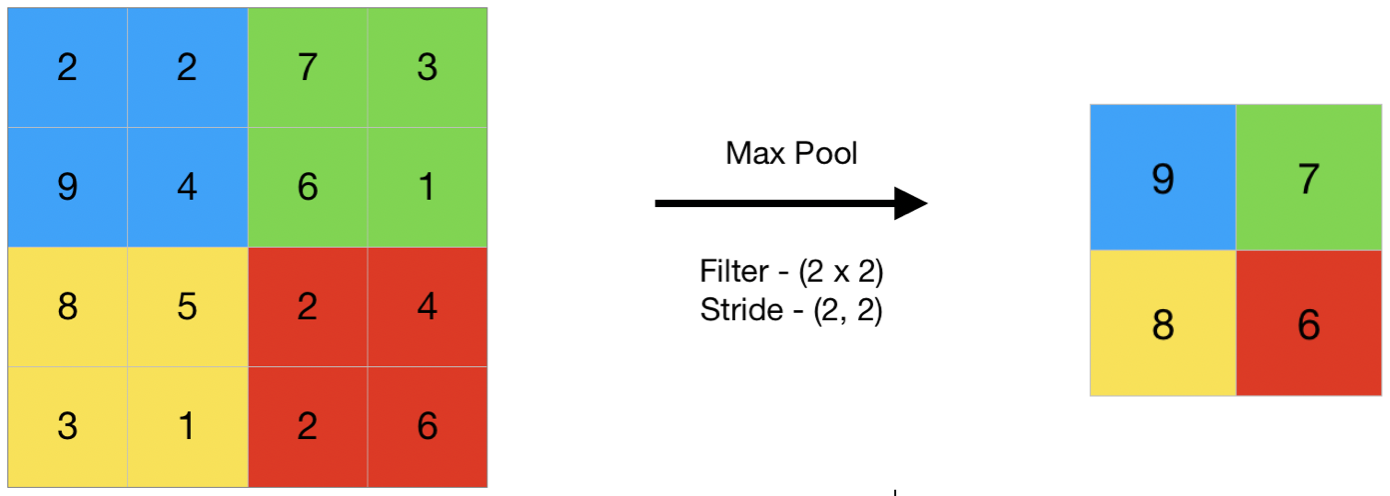
\includegraphics[width=0.6\textwidth]{images/max_pooling_operation.png}
	\captionof{figure}{Minh họa hoạt động của Max Pooling. Một cửa sổ $2 \times 2$ trượt trên bản đồ đặc trưng. Tại mỗi vị trí, giá trị lớn nhất được chọn để đưa vào bản đồ đầu ra, làm giảm kích thước không gian đi một nửa.}
	\label{fig:max_pooling_operation}
\end{center}
% Keyword gợi ý: max pooling cnn, max pooling example, pooling layer explained

\subsubsection{Average Pooling}
\label{subsubsec:average_pooling}
\textbf{Cơ chế hoạt động:} Tương tự như Max Pooling, nhưng thay vì lấy giá trị lớn nhất, nó lấy giá trị \textbf{trung bình (average)} của tất cả các giá trị trong cửa sổ.
\[
\begin{pmatrix}
	1 \& 7 \& 2 \& 4 \\
	8 \& 5 \& 3 \& 6 \\
	3 \& 1 \& 9 \& 2 \\
	5 \& 2 \& 4 \& 8
\end{pmatrix}
\xrightarrow{\text{2x2 Average Pooling, Stride 2}}
\begin{pmatrix}
	5.25 \& 3.75 \\
	2.75 \& 5.75
\end{pmatrix}
\]
Trong lịch sử, Average Pooling đã được sử dụng (ví dụ trong LeNet-5), nhưng thực nghiệm cho thấy Max Pooling thường cho kết quả tốt hơn trong việc trích xuất các đặc trưng phân biệt cho các bài toán phân loại. Average Pooling có xu hướng làm "mờ" các đặc trưng, trong khi Max Pooling giữ lại những tín hiệu mạnh nhất.

\subsubsection{Global Pooling}
\label{subsubsec:global_pooling}
Đây là một dạng pooling đặc biệt, thường được sử dụng ở cuối phần trích xuất đặc trưng của mạng (trước các lớp fully-connected). Thay vì trượt một cửa sổ nhỏ, Global Pooling áp dụng phép toán trên \textbf{toàn bộ} một bản đồ đặc trưng.

\textbf{Cơ chế hoạt động:}
\begin{itemize}
	\item \textbf{Global Average Pooling (GAP):} Dạng phổ biến nhất. Đối với mỗi bản đồ đặc trưng (kích thước $H \times W$), nó tính giá trị trung bình của tất cả $H \times W$ pixel, tạo ra một giá trị duy nhất. Nếu input có kích thước $H \times W \times C$, output của GAP sẽ là một vector $1 \times 1 \times C$.
	\item \textbf{Global Max Pooling (GMP):} Tương tự, nhưng lấy giá trị lớn nhất trên toàn bộ bản đồ đặc trưng.
\end{itemize}

\textbf{Vai trò và Ưu điểm:} Global Average Pooling là một sự thay thế cực kỳ hiệu quả cho việc "làm phẳng" (flatten) các bản đồ đặc trưng và kết nối chúng với các lớp fully-connected lớn.
\begin{itemize}
	\item \textbf{Giảm mạnh số lượng tham số:} Nó loại bỏ hoàn toàn các tham số khổng lồ của các lớp fully-connected truyền thống, giúp giảm đáng kể nguy cơ overfitting.
	\item \textbf{Tăng cường khả năng diễn giải:} GAP tạo ra một tương ứng trực tiếp giữa các bản đồ đặc trưng và các lớp (categories). Mỗi kênh trong bản đồ đặc trưng trước tầng GAP có thể được xem như một ``bản đồ độ tin cậy của lớp'' (class confidence map). Đây là nền tảng cho các kỹ thuật trực quan hóa như Class Activation Mapping (CAM).
\end{itemize}

\begin{center}
	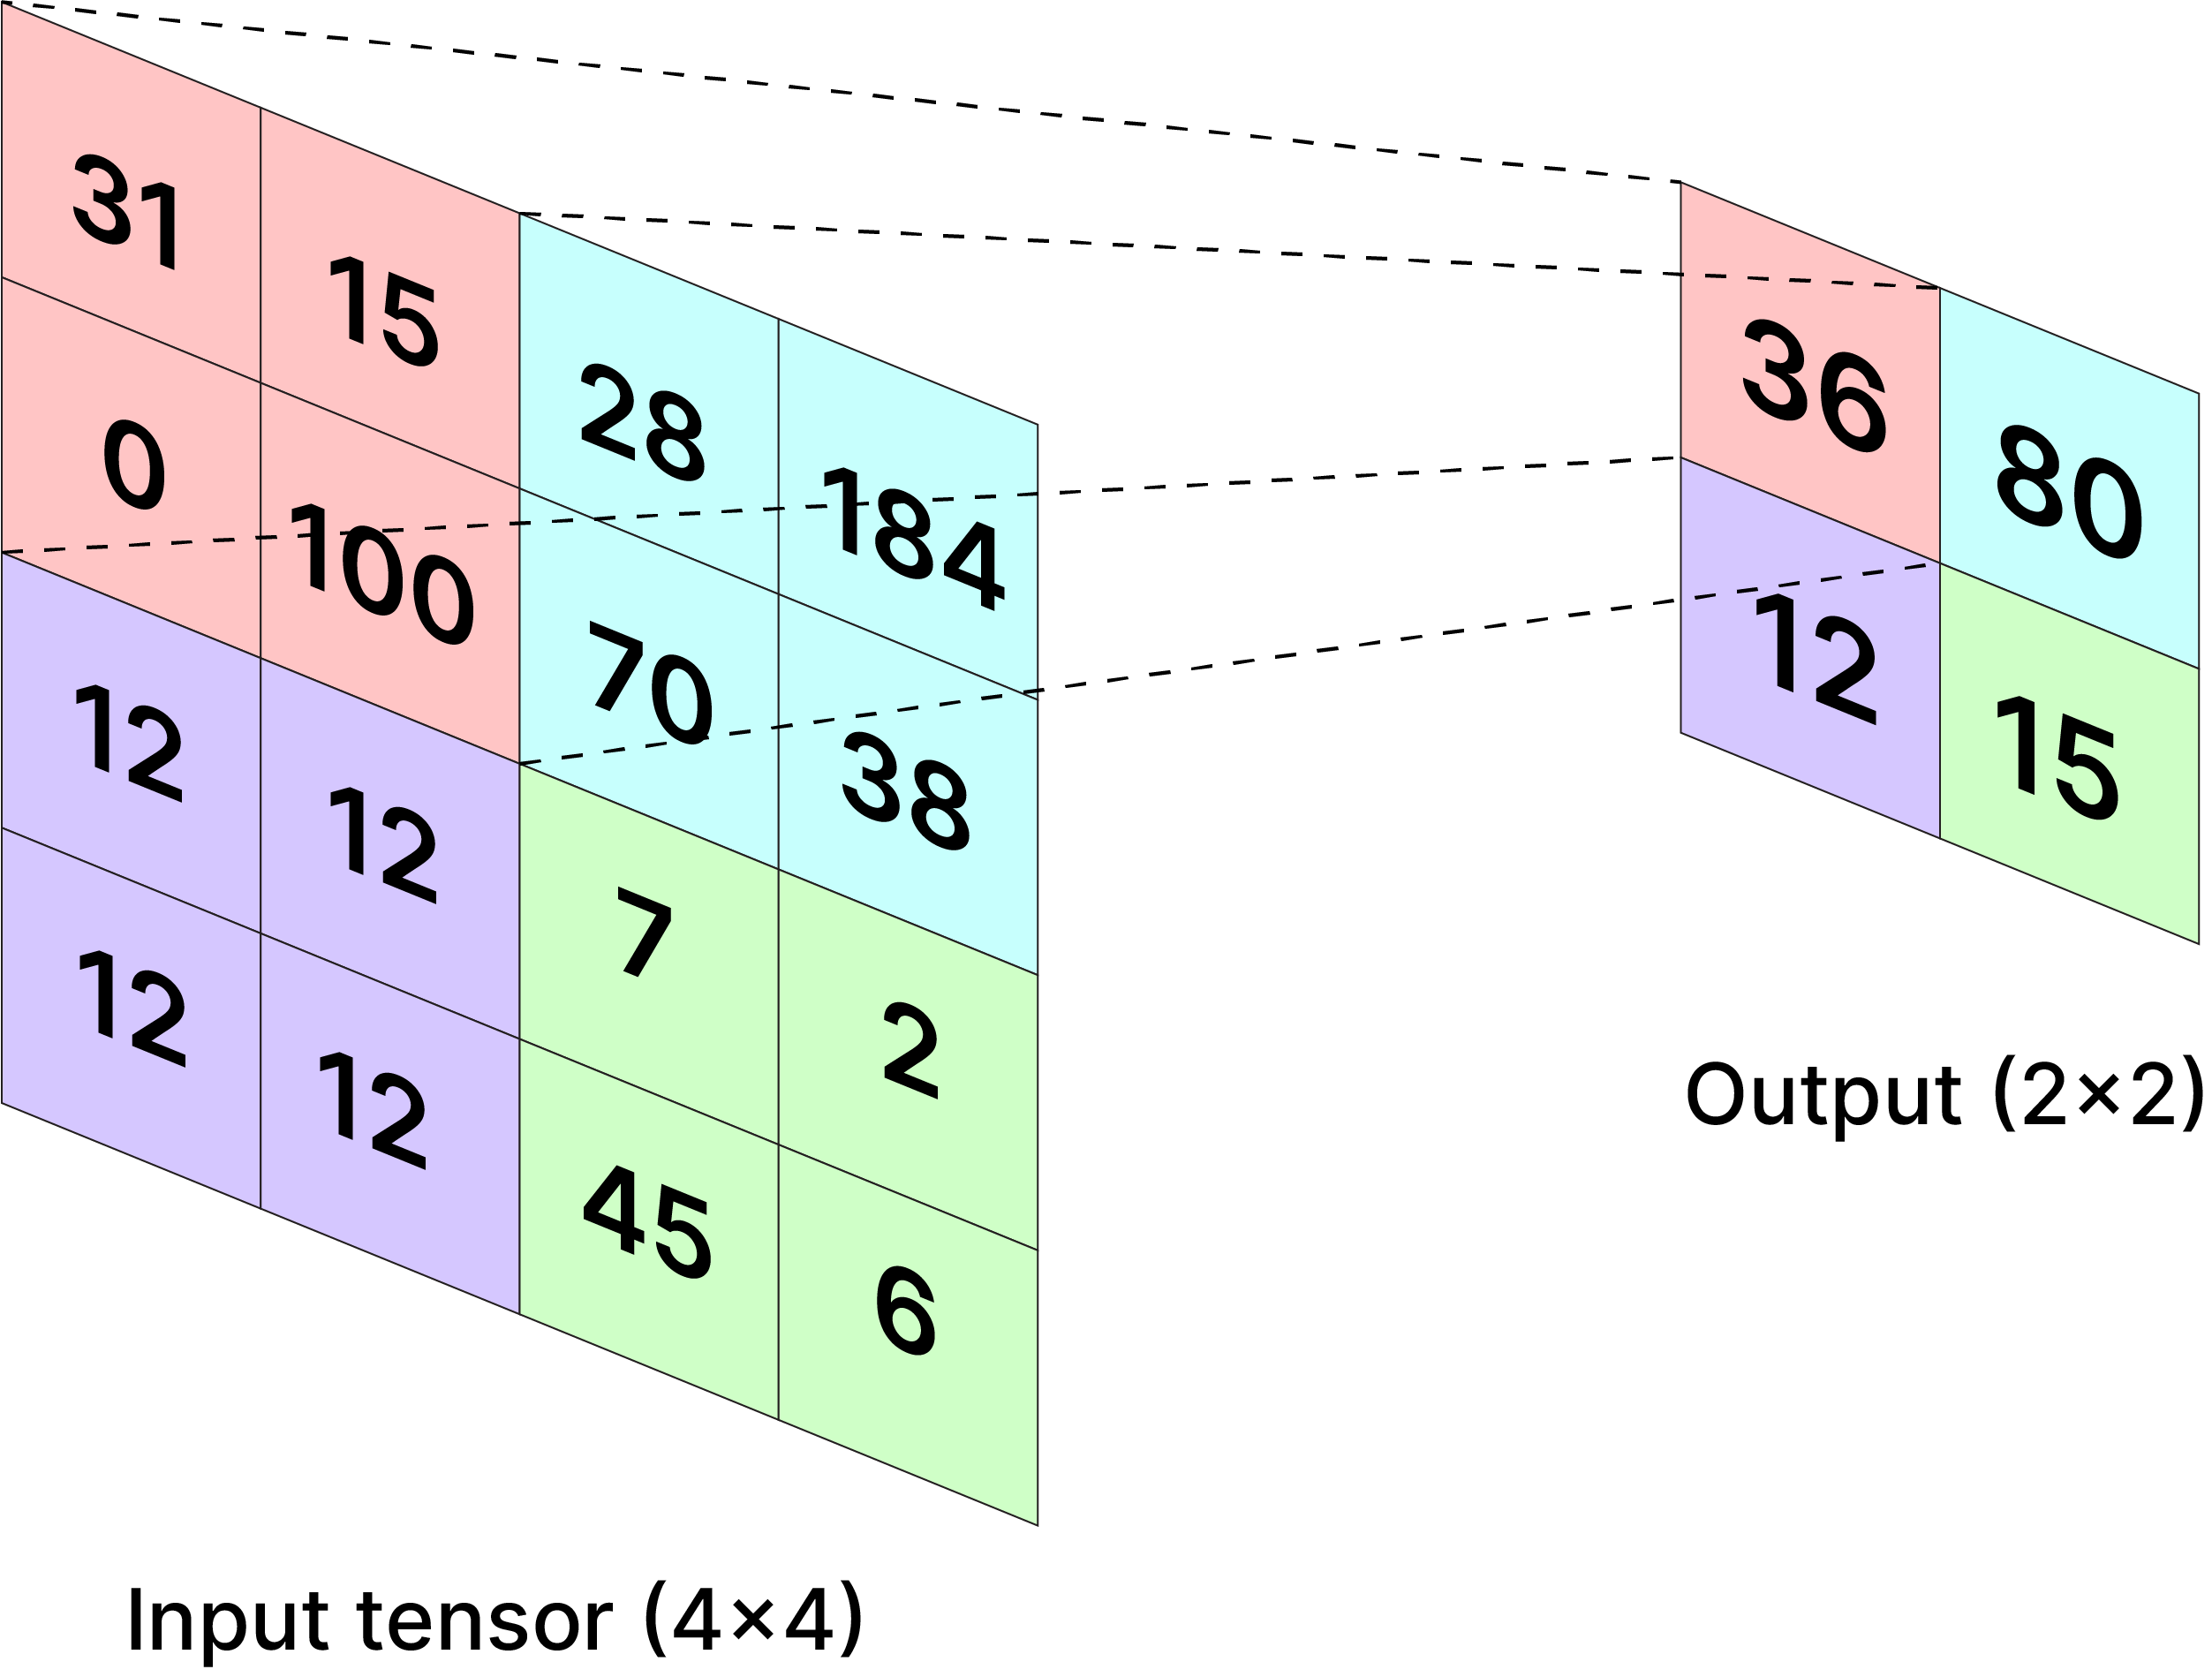
\includegraphics[width=0.9\textwidth]{images/global_average_pooling.png}
	\captionof{figure}{Minh họa Global Average Pooling (GAP). Toàn bộ mỗi kênh đặc trưng (feature map) được thu gọn thành một giá trị duy nhất (giá trị trung bình), biến một khối $H \times W \times C$ thành một vector $1 \times 1 \times C$.}
	\label{fig:global_average_pooling}
\end{center}
% Keyword gợi ý: global average pooling, gap cnn, flatten vs global average pooling

\begin{table}[h!]
	\centering
	\caption{So sánh các loại Pooling}
	\label{tab:pooling_comparison}
	\begin{tabular}{|l|p{4cm}|p{4cm}|p{4cm}|}
		\hline
		\textbf{Tiêu chí} & \textbf{Max Pooling} & \textbf{Average Pooling} & \textbf{Global Average Pooling} \\
		\hline
		\textbf{Phép toán} & Lấy giá trị lớn nhất trong một vùng cục bộ. & Lấy giá trị trung bình trong một vùng cục bộ. & Lấy giá trị trung bình trên toàn bộ bản đồ đặc trưng. \\
		\hline
		\textbf{Mục đích chính} & Giảm chiều, tạo bất biến tịnh tiến cục bộ, giữ lại đặc trưng mạnh nhất. & Giảm chiều, tạo biểu diễn mượt hơn. & Thay thế các lớp fully-connected, giảm tham số, chống overfitting. \\
		\hline
		\textbf{Ưu điểm} & Hiệu quả cho phân loại, giữ lại thông tin quan trọng. & Hoạt động ổn định. & Giảm overfitting mạnh mẽ, tăng khả năng diễn giải. \\
		\hline
		\textbf{Ứng dụng tiêu biểu} & Các lớp trung gian trong hầu hết các mạng CNN. & Ít phổ biến hơn, đôi khi dùng trong các kiến trúc đặc biệt. & Thường ở cuối các mạng hiện đại (ResNet, Inception) trước lớp phân loại. \\
		\hline
	\end{tabular}
\end{table}

\subsection{Activation Functions: Đưa Tính Phi tuyến vào Mạng}
\label{subsec:activation_functions}

Cho đến nay, chúng ta đã thảo luận về hai phép toán cốt lõi: tích chập và pooling. Cả hai đều là các phép toán tuyến tính (linear operations). Một phép tích chập về bản chất là một tổng có trọng số. Một phép pooling (cả max và average) cũng là một phép toán tuyến tính cục bộ.

\begin{mdframed}[style=infobox]
	\textbf{Vấn đề của sự Tuyến tính}
	
	Hãy tưởng tượng điều gì sẽ xảy ra nếu chúng ta xếp chồng nhiều lớp tích chập và pooling lên nhau mà không có gì ở giữa. Về mặt toán học, một chuỗi các phép biến đổi tuyến tính liên tiếp (ví dụ: áp dụng ma trận A, rồi ma trận B, rồi ma trận C) chỉ tương đương với một phép biến đổi tuyến tính duy nhất (áp dụng ma trận $D = C \cdot B \cdot A$).
	
	Điều này có nghĩa là, một mạng "sâu" gồm toàn các lớp tuyến tính sẽ không có khả năng biểu diễn mạnh hơn một mạng "nông" chỉ có một lớp duy nhất. Nó không thể học được các mối quan hệ phức tạp, phi tuyến vốn có trong dữ liệu hình ảnh (ví dụ: mối quan hệ giữa các bộ phận để tạo thành một khuôn mặt). Toàn bộ sức mạnh của kiến trúc sâu sẽ bị lãng phí.
\end{mdframed}

Để phá vỡ sự tuyến tính này và mở khóa khả năng học các hàm phức tạp, chúng ta cần chèn một thành phần \textbf{phi tuyến (non-linear)} vào giữa các lớp. Thành phần đó chính là \textbf{hàm kích hoạt (activation function)}. Nó được áp dụng theo từng phần tử (element-wise) lên bản đồ đặc trưng đầu ra của một lớp tích chập.

\subsubsection{Các Hàm Kích hoạt Sơ khai: Sigmoid và Tanh}
\label{subsubsec:early_activations}
Trong những ngày đầu của mạng nơ-ron, các hàm kích hoạt phổ biến được lấy cảm hứng từ sinh học và có dạng "S" (sigmoidal).
\begin{description}
	\item[Sigmoid (Logistic):] Hàm này nén một giá trị thực bất kỳ vào khoảng $(0, 1)$.
	\begin{equation}
		\sigma(x) = \frac{1}{1 + e^{-x}}
	\end{equation}
	Nó từng rất phổ biến vì có thể được diễn giải như một "xác suất kích hoạt" của một nơ-ron. Tuy nhiên, nó có hai nhược điểm lớn:
	\begin{itemize}
		\item \textbf{Gây ra Vấn đề Suy giảm Gradient (Vanishing Gradient Problem):} Đạo hàm của hàm sigmoid có giá trị lớn nhất là 0.25 tại $x=0$ và tiến rất nhanh về 0 khi $|x|$ tăng. Khi lan truyền ngược qua nhiều lớp, các gradient sẽ bị nhân với các giá trị nhỏ này, khiến cho gradient ở các lớp đầu tiên trở nên gần như bằng 0. Kết quả là các lớp này gần như không học được gì.
		\item \textbf{Output không Zero-centered:} Output của sigmoid luôn dương. Điều này có thể làm chậm quá trình hội tụ của thuật toán tối ưu hóa.
	\end{itemize}
	
	\item[Tanh (Hyperbolic Tangent):] Hàm này nén một giá trị thực vào khoảng $(-1, 1)$.
	\begin{equation}
		\tanh(x) = \frac{e^x - e^{-x}}{e^x + e^{-x}} = 2\sigma(2x) - 1
	\end{equation}
	Tanh giải quyết được vấn đề output không zero-centered, giúp quá trình hội tụ nhanh hơn sigmoid. Tuy nhiên, nó vẫn bị vấn đề suy giảm gradient, mặc dù mức độ có nhẹ hơn một chút (đạo hàm lớn nhất là 1 tại $x=0$).
\end{description}
Do vấn đề suy giảm gradient, Sigmoid và Tanh ngày nay rất hiếm khi được sử dụng trong các lớp ẩn của các mạng sâu.

\begin{center}
	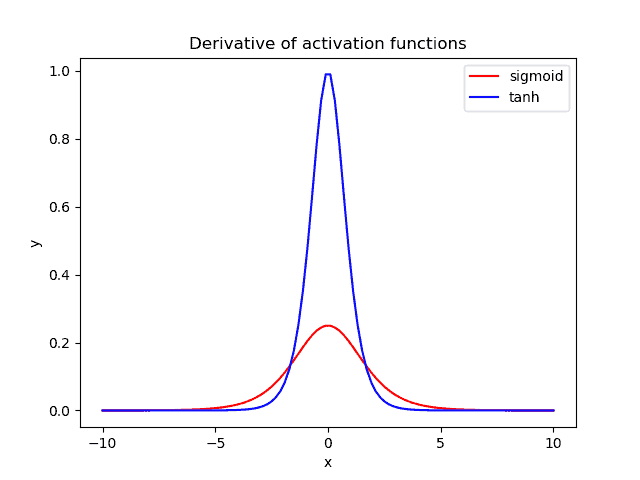
\includegraphics[width=0.9\textwidth]{images/sigmoid_tanh_derivatives.png}
	\captionof{figure}{(Trái) Đồ thị hàm Sigmoid và Tanh. (Phải) Đồ thị đạo hàm của chúng. Có thể thấy đạo hàm của cả hai hàm đều tiến nhanh về 0 khi giá trị đầu vào ra xa khỏi 0, gây ra hiện tượng suy giảm gradient.}
	\label{fig:sigmoid_tanh_derivatives}
\end{center}
% Keyword gợi ý: sigmoid tanh derivative vanishing gradient

\subsubsection{Cuộc cách mạng ReLU (Rectified Linear Unit)}
\label{subsubsec:relu_revolution}
Sự ra đời của hàm Kích hoạt Tuyến tính Chỉnh lưu (ReLU) là một trong những bước ngoặt quan trọng nhất cho phép huấn luyện các mạng nơ-ron sâu một cách hiệu quả. Công thức của nó đơn giản đến bất ngờ:
\begin{equation}
	\text{ReLU}(x) = \max(0, x) = 
	\begin{cases} 
		x & \text{if } x > 0 \\
		0 & \text{if } x \le 0
	\end{cases}
\end{equation}
Sự đơn giản này mang lại những lợi ích to lớn:
\begin{enumerate}
	\item \textbf{Hiệu quả tính toán vượt trội:} Không có các phép tính mũ (`exp`) đắt đỏ như Sigmoid hay Tanh. Phép toán chỉ là một phép so sánh đơn giản với 0, giúp tăng tốc đáng kể cả quá trình huấn luyện và suy luận.
	\item \textbf{Khắc phục Vấn đề Suy giảm Gradient (phần lớn):} Đối với mọi giá trị đầu vào dương ($x>0$), đạo hàm của ReLU là một hằng số bằng 1. Điều này cho phép gradient được lan truyền ngược qua nhiều lớp mà không bị suy giảm, là chìa khóa để huấn luyện các mạng rất sâu.
	\item \textbf{Tạo ra sự Thưa thớt (Sparsity):} Bằng cách đặt tất cả các giá trị âm về 0, ReLU tạo ra các biểu diễn thưa thớt. Tức là tại một thời điểm, chỉ một phần các nơ-ron trong mạng được "kích hoạt". Điều này có thể làm giảm sự phụ thuộc lẫn nhau giữa các nơ-ron và có tác dụng như một hình thức chính quy hóa (regularization).
\end{enumerate}
Tuy nhiên, ReLU không hoàn hảo. Nó có một điểm yếu được gọi là \textbf{"Dying ReLU Problem"}. Nếu một nơ-ron, vì một lý do nào đó (ví dụ: khởi tạo trọng số không tốt hoặc learning rate quá cao), luôn nhận giá trị đầu vào âm, thì đầu ra của nó sẽ luôn là 0. Do đó, đạo hàm tại điểm đó cũng luôn là 0. Nơ-ron này sẽ không bao giờ cập nhật lại trọng số của nó nữa và trở nên "chết", không còn đóng góp gì cho mạng.

\subsubsection{Gia đình ReLU: Các nỗ lực Cải tiến}
\label{subsubsec:relu_family}
Để giải quyết vấn đề "Dying ReLU", một loạt các biến thể đã được đề xuất, tạo thành một "gia đình" các hàm kích hoạt dựa trên ReLU.
\begin{description}
	\item[Leaky ReLU:] Ý tưởng rất đơn giản: thay vì bằng 0, cho phép một "dòng rò" (leak) nhỏ ở phần âm.
	\begin{equation}
		\text{LeakyReLU}(x) = \max(\alpha x, x) = 
		\begin{cases} 
			x & \text{if } x > 0 \\
			\alpha x & \text{if } x \le 0
		\end{cases}
	\end{equation}
	trong đó $\alpha$ là một hằng số nhỏ, thường là 0.01. Điều này đảm bảo rằng các nơ-ron luôn có một gradient nhỏ khác 0, giúp chúng không bị "chết".
	
	\item[Parametric ReLU (PReLU):] Thay vì chọn một giá trị $\alpha$ cố định, tại sao không để mạng tự học giá trị tốt nhất? PReLU biến $\alpha$ thành một tham số có thể học được.
	
	\item[Exponential Linear Unit (ELU):] ELU sử dụng một hàm mũ cho phần âm, tạo ra một đường cong mượt hơn và có thể đẩy giá trị trung bình của các kích hoạt về gần 0, giúp tăng tốc độ học.
	\begin{equation}
		\text{ELU}(x) = 
		\begin{cases} 
			x & \text{if } x > 0 \\
			\alpha (e^x - 1) & \text{if } x \le 0
		\end{cases}
	\end{equation}
\end{description}

\begin{center}
	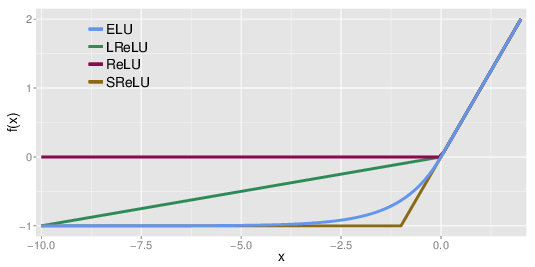
\includegraphics[width=0.7\textwidth]{images/relu_family_plot.png}
	\captionof{figure}{So sánh đồ thị của ReLU và các biến thể của nó (Leaky ReLU, ELU). Các biến thể này đều có giá trị và gradient khác 0 ở phần âm để giải quyết vấn đề "Dying ReLU".}
	\label{fig:relu_family_plot}
\end{center}
% Keyword gợi ý: relu leaky relu elu plot, relu family activation functions

\subsubsection{Các Hàm Kích hoạt Hiện đại: Mượt mà và Hiệu quả hơn}
\label{subsubsec:modern_activations}
Trong những năm gần đây, đặc biệt với sự trỗi dậy của các kiến trúc Transformer, các nhà nghiên cứu đã phát triển các hàm kích hoạt mượt (smooth) và không đơn điệu (non-monotonic), cho thấy hiệu năng vượt trội hơn ReLU trong nhiều tác vụ.

\begin{description}
	\item[GELU (Gaussian Error Linear Unit):] Trở thành tiêu chuẩn trong các mô hình Transformer như BERT và GPT. GELU có thể được xem là một phiên bản "xác suất" của ReLU.
	\begin{equation}
		\text{GELU}(x) = x \cdot \Phi(x)
	\end{equation}
	trong đó $\Phi(x)$ là hàm phân phối tích lũy (CDF) của phân phối chuẩn Gauss. Trực giác của nó là: nó làm giảm trọng số của một kích hoạt $x$ dựa trên xác suất nó nhỏ hơn các kích hoạt khác dưới một phân phối chuẩn. GELU là một hàm mượt và không đơn điệu, và có một phép xấp xỉ nhanh thường được dùng trong thực tế:
	\begin{equation}
		\text{GELU}(x) \approx 0.5x \left(1 + \tanh\left[\sqrt{2/\pi}(x + 0.044715x^3)\right]\right)
	\end{equation}
	
	\item[Swish:] Một hàm được tìm ra thông qua tìm kiếm kiến trúc tự động (automated architecture search).
	\begin{equation}
		\text{Swish}(x) = x \cdot \sigma(\beta x)
	\end{equation}
	trong đó $\sigma$ là hàm sigmoid và $\beta$ là một hằng số hoặc một tham số có thể học. Khi $\beta=1$, nó được gọi là SiLU (Sigmoid-weighted Linear Unit). Swish có hình dạng rất giống GELU và thường cho hiệu năng tương đương hoặc tốt hơn.
	
	\item[Mish:] Một hàm kích hoạt mượt và tự chính quy hóa (self-regularized), được báo cáo là vượt qua Swish và ReLU trên nhiều bộ dữ liệu.
	\begin{equation}
		\text{Mish}(x) = x \cdot \tanh(\text{softplus}(x))
	\end{equation}
	trong đó $\text{softplus}(x) = \ln(1 + e^x)$. Mish có một độ lõm nhỏ ở phần âm, một đặc tính không đơn điệu giúp cải thiện luồng gradient.
\end{description}

\begin{center}
	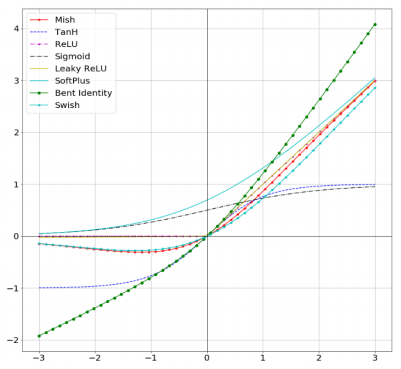
\includegraphics[width=0.9\textwidth]{images/modern_activations_plot.png}
	\captionof{figure}{So sánh đồ thị các hàm kích hoạt hiện đại: ReLU, GELU, Swish, và Mish. Có thể thấy các hàm hiện đại đều là các xấp xỉ mượt của ReLU. Đồ thị đạo hàm của chúng cho thấy một luồng gradient mượt mà hơn so với "bước nhảy" đột ngột của ReLU.}
	\label{fig:modern_activations_plot}
\end{center}
% Keyword gợi ý: relu gelu swish mish plot, modern activation functions

\subsubsection{Lựa chọn Hàm kích hoạt nào?}
Với rất nhiều lựa chọn, câu hỏi đặt ra là nên dùng hàm nào. Dưới đây là một vài quy tắc kinh nghiệm:
\begin{itemize}
	\item \textbf{ReLU là lựa chọn mặc định an toàn nhất.} Nó nhanh, hiệu quả và hoạt động tốt trên phần lớn các kiến trúc CNN. Hãy luôn bắt đầu với ReLU.
	\item Nếu bạn gặp vấn đề với "Dying ReLU", hãy thử \textbf{Leaky ReLU} hoặc các biến thể của nó.
	\item Nếu bạn đang làm việc với các kiến trúc rất hiện đại (như Transformer) hoặc muốn tối ưu hóa để đạt hiệu năng cao nhất có thể, hãy thử nghiệm với \textbf{GELU, Swish, hoặc Mish}.
	\item Đối với các ứng dụng trên thiết bị di động/nhúng, các phiên bản "cứng" như \textbf{Hard Swish} (được dùng trong MobileNetV3) là lựa chọn tốt để cân bằng giữa độ chính xác và tốc độ suy luận.
\end{itemize}
Cuối cùng, không có một hàm kích hoạt nào là tốt nhất cho mọi bài toán. Việc lựa chọn tối ưu thường được xác định thông qua thực nghiệm.

\section*{Tài liệu tham khảo}
\begin{itemize}
	\item[1] LeCun, Y., Bottou, L., Bengio, Y., \& Haffner, P. (1998). Gradient-based learning applied to document recognition. \textit{Proceedings of the IEEE}, 86(11), 2278-2324. (Paper kinh điển giới thiệu LeNet-5, một trong những kiến trúc CNN thành công đầu tiên, đặt nền móng cho việc sử dụng các lớp Convolution, Pooling và các hàm kích hoạt như Tanh).
	\item[2] Krizhevsky, A., Sutskever, I., \& Hinton, G. E. (2012). ImageNet classification with deep convolutional neural networks. In \textit{Advances in neural information processing systems (NIPS)}. (Paper giới thiệu AlexNet, đã phổ biến hóa việc sử dụng ReLU và chứng minh hiệu quả vượt trội của nó so với Tanh, khởi đầu cuộc cách mạng ReLU).
	\item[3] Nair, V., \& Hinton, G. E. (2010). Rectified linear units improve restricted boltzmann machines. In \textit{Proceedings of the 27th International Conference on Machine Learning (ICML)}. (Một trong những bài báo đầu tiên đề xuất và phân tích sâu về hàm ReLU).
	\item[4] Maas, A. L., Hannun, A. Y., \& Ng, A. Y. (2013). Rectifier nonlinearities improve neural network acoustic models. In \textit{Proc. ICML}. (Bài báo giới thiệu Leaky ReLU như một giải pháp cho vấn đề "Dying ReLU").
	\item[5] He, K., Zhang, X., Ren, S., \& Sun, J. (2015). Delving deep into rectifiers: Surpassing human-level performance on imagenet classification. In \textit{Proceedings of the IEEE international conference on computer vision (ICCV)}. (Giới thiệu Parametric ReLU - PReLU).
	\item[6] Clevert, D. A., Unterthiner, T., \& Hochreiter, S. (2015). Fast and accurate deep network learning by exponential linear units (ELUs). \textit{arXiv preprint arXiv:1511.07289}. (Giới thiệu hàm ELU).
	\item[7] Hendrycks, D., \& Gimpel, K. (2016). Gaussian error linear units (GELUs). \textit{arXiv preprint arXiv:1606.08415}. (Giới thiệu hàm GELU, sau này được sử dụng rộng rãi trong Transformer).
	\item[8] Ramachandran, P., Zoph, B., \& Le, Q. V. (2017). Searching for activation functions. \textit{arXiv preprint arXiv:1710.05941}. (Giới thiệu hàm Swish, được tìm ra bằng phương pháp tìm kiếm tự động).
	\item[9] Misra, D. (2019). Mish: A self regularized non-monotonic activation function. \textit{arXiv preprint arXiv:1908.08681}. (Giới thiệu hàm Mish).
	\item[10] Lin, M., Chen, Q., \& Yan, S. (2013). Network in network. \textit{arXiv preprint arXiv:1312.4400}. (Paper tiên phong trong việc đề xuất sử dụng Global Average Pooling để thay thế các lớp Fully-Connected, một ý tưởng quan trọng trong các kiến trúc CNN hiện đại).
\end{itemize}
